% !TEX root = ../thesis_main.tex
\chapter{Introduction}
%%%%%%%%%%%%%%%%%%%%%%%%%%%%%%%%%%%%%%%%%%%%%%%%%%%%%%
%  OPENING
%%%%%%%%%%%%%%%%%%%%%%%%%%%%%%%%%%%%%%%%%%%%%%%%%%%%%%
% why learning from imperfect supervising? motivation based on the human ability. We talk about both HUMAN and MACHINE (to immediately show that we are not going to merely talk about human learning in the reset of the thesis.)
~\todo{fix conflict with Chomsky}
Humans can effortlessly learn about new concepts and solve complex problems from limited, noisy or inconsistent observations and routinely draw successful generalization on them, yet it remains a key challenge for our best machines to learn from imperfect supervision.

This general argument has been advanced under the name ``\emph{poverty of the stimulus}'', proposed by ~\citet{chomsky1980rules}. It suggests that human children can learn something as complex as a natural language from the limited inputs of variable quality and need no evidence for much of the knowledge they bring to the learning process. 
% how to explain human learning considering POS?
To explain this, some researchers postulate the innateness of some knowledge.
%
% since this the very first page of the thesis and this quote is relevant to the general discussion, but not directly to the whole thesis, we can remove this part.
Along with this line, Chomsky noted~\citep{chomsky1980rules}:
\begin{quote}
    ``\emph{My own suspicion is that a central part of what we call “learning” is actually better understood as the growth of cognitive structures along an internally directed course under the triggering and partially shaping effect of the environment.}''\footnote{There has been a long discussion between rationalists and empiricists. Here, we just want to draw a connection between the problem of \emph{poverty of stimulus} in both human and machine learning process.}
\end{quote}

% back to machine learning
Like human, machines are confronted with the intriguing problem of the poverty of stimulus, although capturing such human-level learning abilities, given imperfect supervisions, in machines remains a fundamental challenge~\citep{lake2017building} in many domains. 
%
% pos in machines and the necessity of {data-driven + innately primed} learning 
Similar arguments have been put forward in machine learning to deal with the problem of \emph{poverty of stimulus} and more generally the \emph{generalization} of learning algorithms, that a learner that makes no prior assumptions has no rational basis for generalizing over unseen instances~\citep{Mitchell:1997:ML}, which implies the futility of unbiased learning. %~\footnote{In fact, learner with no bias does not exist~\todo{cite}~\citep{}}.

%%%%%%%%%%%%%%%%%%%%%%%%%%%%%%%%%%%%%%%%%%%%%%%%%%%%%%
%  FIRST PART OF THE TITLE: "LEARNING WITH IMPERFECT SUPERVISION [...]"
%%%%%%%%%%%%%%%%%%%%%%%%%%%%%%%%%%%%%%%%%%%%%%%%%%%%%%
% What is important supervising and why learning with imperfect supervision?
Most of the today's success of data-driven machine learning systems depend on the availability of massive amount of high-quality labeled data and in many cases, the more data you have, the more accurate your model will be~\citep{halevy2009unreasonable,sun2017revisiting}. 
However, in many real-world applications, such training data is not available.
This highlights the increasing need for building models with the ability to learn complex tasks with \emph{imperfect supervision}. In this thesis, we use ``\emph{imperfect supervision}'' as an umbrella term covering a variety of situations where the learning process is based on imperfect training examples~\citep{zhou2018brief}.

% high level ideas to deal with lack of data
In practice, to deal with data scarcity in many tasks and applications, we can use higher-level approaches to either provide supervision signals for training learning algorithms. 
% a list of alternative approaches
This can be done for instance by
using distant or heuristic supervision~\citep{Deriu2016:SemEval,Severyn:2015:SemEval, Dehghani:2016:SIGIR, dehghani:2018:ICLR, Dehghani:2017:nips_metalearn, Ratner:2016,Rekatsinas:2017,Varma:2017}, 
%
using incidental signals that exist in the data and the environment independently of the tasks and they are co-related to the target tasks~\citep{roth2017incidental}, 
%
providing supervision by specifying constraints that should hold over the output space~\citep{stewart2017label, clarke2010driving}, 
%
applying bootstrapping, self-supervised feature learning, and data augmentation to make statistically efficient reuse of available data~\citep{cubuk2018autoaugment, dosovitskiy2016discriminative,donahue2016adversarial},
%
using transfer learning to generalize knowledge across domains~\citep{Ruder:2019},
%
using active learning and response-based supervision in which the model receives feedback from interacting with an environment~\citep{clarke2010driving,riezler2014response},
%
introducing a form of structured prior knowledge~\citep{Dehghani:CIKM2016:long,Dehghani:2016:ICTIR}, 
%
zero/one/few-shot learning~\citep{vinyals2016matching,finn2017model,snell2017prototypical,socher2013zero},
%
exploiting noisy and inaccurate labels~\citep{Vahdat:2017, Lee:2013,Hinton:2015,Brodley:1999,reed2014training, Patrini:2016, patrini2016loss,malach2017decoupling}, 
%
and injecting inductive biases into algorithms to generalize better on unobserved data~\citep{cohen2016group, cohen2016steerable, Dehghani:ICLR:2019}.

%%%%%%%%%%%%%%%%%%%%%%%%%%%%%%%%%%%%%%%%%%%%%%%%%%%%%%
%  SECOND PART OF THE TITLE: "[...] FOR LANGUAGE UNDERSTANDING"
%%%%%%%%%%%%%%%%%%%%%%%%%%%%%%%%%%%%%%%%%%%%%%%%%%%%%%
% why language understanding?
The reason that we focus on language understanding is that understanding language is an extraordinary cognitive ability of human. 
%
There have been several attempts to check if nonhuman animals can acquire language~\citep{pepperberg2017animal}, like Project Nim\footnote{\url{https://nl.wikipedia.org/wiki/Project_Nim}}, a research project that was mounted in the 1970s to determine whether a chimpanzee, named Nim Chimpsky, raised in close contact with humans could develop a limited language. Regardless of the fact that at the end Nim was using language to communicate or simply going through a bag of tricks to get things, it was much more limited compared to what human child can develop in the early years. 
%
This indicates that achieving human-level understanding and generating of language, would not be an easy goal for machines either.

Improving machines on understanding of language and studying how to solve language tasks can help moving toward detecting core cognitive ingredients of human-level intelligence and get closer to the bigger goal of creating artificial general intelligence.

Minsky? ~\todo{improving the learning not tasks --> abstract biases}
% a list of language understanding tasks that we have in this thesis
Here, in this thesis, we study the effectiveness of our proposed learning algorithms on a wide range of sequence modeling and language understanding tasks, including:
% 
assessing relevance for ranking (Chapter~\ref{chap:2}, \ref{chap:4}, and \ref{chap:5}), 
%
(pseudo)-relevance feedback for document ranking(Chapter~\ref{chap:2}), 
%
Machine Translation (Chapter~\ref{chap:5}), 
%
natural language reasoning -- bAbI tasks~\citep{weston2015towards} (Chapter~\ref{chap:5}), 
%
broad context language modeling~\citep{paperno2016lambada} (Chapter~\ref{chap:5}), 
%
contextual suggestion~\citep{hashemioverview} (Chapter~\ref{chap:3}), 
%
open-domain question answering (Chapter~\ref{chap:5}), 
%
modeling hierarchical structure in natural language -- subject-verb agreement task~\citep{linzen2016assessing} (Chapter~\ref{chap:3}), 
%
text classification (Chapter~\ref{chap:3}), 
%
sentiment analysis (Chapter~\ref{chap:5}), 
%
learning to execute computer programs~\citep{ZS14} (Chapter~\ref{chap:5}), 
%
and a set of algorithmic tasks~\citep{neural_gpu} (Chapter~\ref{chap:5}).

Besides the challenges of learning from imperfect supervision in many of these tasks, some of them are difficult tasks that, for instance, require learning rich representations, or capturing complex underlying relations, or detecting and understanding abstract concepts and reasoning about them.
%
Although we mainly focus on sequence modeling and language-related tasks and evaluate our proposed ideas on these tasks, some of the proposed models in this thesis have no strong tie to language and can be easily extended to other domains like computer vision.

%%%%%%%%%%%%%%%%%%%%%%%%%%%%%%%%%%%%%%%%%%%%%%%%%%%%%%
%  CLOSING THE INTRO SECTION IF THE INTRODUCTION CHAPTER!
%%%%%%%%%%%%%%%%%%%%%%%%%%%%%%%%%%%%%%%%%%%%%%%%%%%%%%
\medskip
In this thesis, to overcome the problem of poverty of stimulus for learning algorithms, we focus on  i) \emph{employing the prior knowledge}, ii) \emph{augmenting data and meta-learning how to better use the data}, and iii) \emph{introducing inductive biases to learning algorithms}, all to improve the learning process. We believe these approaches are great ways to move toward better machine learning systems that are able to generalize over observed imperfect training signals and as ~\citet{Mitchell80theneed} states in his paper:
\begin{quote}
``\emph{If biases and initial knowledge are at the heart of the ability to generalize beyond observed data, then efforts to study machine learning must focus on the combined use of prior knowledge, biases, and observation in guiding the learning process. It would be wise to make the biases and their use in controlling learning just as explicit as past research has made their observations and use.}''
\end{quote}
There are many domains and applications that suffer from the lack of a large amount of high quality labeled data. We believe building machine learning systems that can learn with imperfect supervision can be considered as a part of the bigger effort to democratize AI by making it dramatically easier to extend AI-powered systems to those domains with limited or noisy data.



\section{Problem Description and Research Questions}
Curating a large amount of high quality labeled training data has become the primary bottleneck in developing new methods and applications in machine learning. 
In general supervised learning scenario, each training example, which is used as the supervision signal, consist of a \emph{feature vector} (also called data instance) and a \emph{label}. However, in many domains and application, there is an imperfection in the supervision signal. Here, in this thesis, we focus on two main problems: dealing with \emph{noisy} training data or/and \emph{limited} training data. 
We formulate the main research question that is addressed in this thesis as follows:
\resq{main}

Based on the above terminology, i.e. features versus label and noisy versus limited, we can presume different types of imperfections in the supervision signal. In each part of this thesis, we target one or some of these types and proposed ideas that can improve the learning process with whit that type of imperfection in supervision. 

Figure~\ref{fig:thesis_parts} summarizes the different types of supervision we consider in each part of these thesis.
\begin{figure}[t]
    \centering
    \begin{subfigure}[b]{0.32\textwidth}
    \centering
        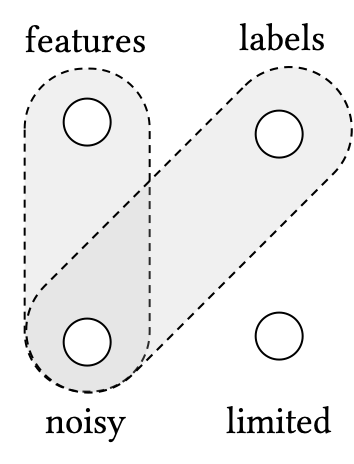
\includegraphics[width=0.55\linewidth]{01-introduction/figs_and_tables/fig_p1.png}
        \caption{\label{fig:p1}Part I}
    \end{subfigure}
        ~ 
    \begin{subfigure}[b]{0.32\textwidth}
    \centering
        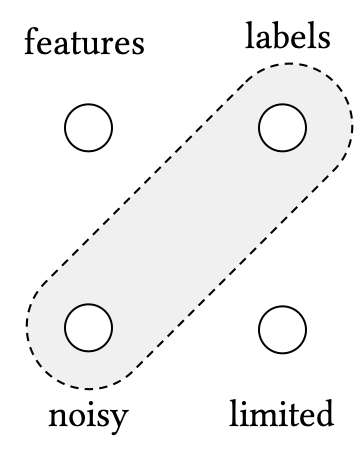
\includegraphics[width=0.55\linewidth]{01-introduction/figs_and_tables/fig_p2.png}
        \caption{\label{fig:p2}Part II}
    \end{subfigure}
        ~ 
    \begin{subfigure}[b]{0.32\textwidth}
    \centering
        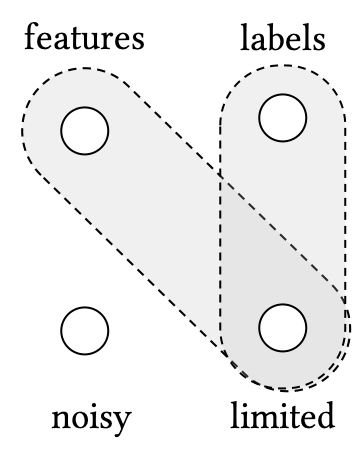
\includegraphics[width=0.55\linewidth]{01-introduction/figs_and_tables/fig_p3.png}
        \caption{\label{fig:p3}Part III}
    \end{subfigure}
\caption{\label{fig:thesis_parts}Type of imperfections in the supervision that we deal with in each art of this thesis.}
\end{figure}

In Part~\ref{part1} of the thesis, we mainly study ideas that address the problem of noisy features. We propose robust models that can deal with non-relevant terms in relevant documents when modeling the notion of relevance in the context of relevance feedback tasks for document ranking. We also propose models that are capable of detecting and ignoring the unstable noisy features that change over time when learning representations from data that evolves over time. We also partly address the problems of noisy labels by modeling the relevance in pseudo-relevance feedback tasks for document ranking, where top-k ranked documents in a retrieval run are assumed as relevant documents, while this assumption does not hold for all cases.

The general approach in the proposed models in Part~\ref{part1} is around the idea of exploring how the structure of the data can be incorporated as prior knowledge to learn representations that are more robust against noise and changes in the data during the time. 
The following research question is the main question that is addressed in Part~\ref{part1} of the thesis:
\resq{p1}
%
In part~\ref{part2} of the thesis, we target the problem of noisy or weak labels. We study how we can develop neural networks that can learn from weakly annotated training examples with the ability to go beyond the imperfection of the weak labels. We study diffident architectural choices and objective functions for neural ranking models to find a more noise tolerant model when learning from pseudo-labels.  We also introduce some ideas that meta-learn the fidelity of weakly annotated labels and modulate the learning process based on the fidelity scores of weakly labeled examples.
In this part, we address the following research question:
\resq{p2}
%
In part~\ref{part3}, we deal with the problem of limited labeled data, for instance, the context of bAbI reasoning tasks with 1k training examples where the tasks are complex and data is limited in terms of the number of training examples. We also study the cases that we have a lot of labeled examples, but with limited coverage, which can be seen as the limitation in the diversity of feature vectors. For instance in the context of algorithmic tasks, with the intention of assessing the ability of models on length generalization, we have plenty of training data but the distribution of sample's length in training is totally different from the test set. 
In this part, we investigate the idea of injecting some inductive biases~\footnote{Inductive biases are ``any biases for choosing one generalization over another, other than strict consistency with the observed training samples." as defined by~\citet{Mitchell80theneed}. We elaborate on this at the beginning of Part~\ref{part3}.} into models in order to encode modeling assumptions that help the models to be more data efficient and generalize better.
The main research question that is addressed in Part~\ref{part3} is:
\resq{p3}

In the next section, we present an overview of the thesis and introduce the structure of the content and summarize different chapters in each part of the thesis.

\section{Thesis Overview}
This thesis consists of the introductory matter, followed by five main
chapters that are divided into three parts that are described in the previous section. Finally, it closes off with the Conclusions and Bibliography. 
The following gives a short description of each part and summarizes each chapter: 

\subsection*{PART I: \titleof{p1}}
In this part, we explore how taking the general structured of the data into account can help to estimate representations that capture only the significant features when the data is noisy and highly variant over time. We break our discussions in this part of the thesis into two chapters:

\subsubsection*{Chapter 2: \titleof{c2}}
In this chapter, we address the following research question:
\resq{c2}
We introduce \emph{\swlm} (\acswlm)~\citep{Dehghani:2016:SIGIR} to learn a representation for a set of textual entities, where this representation captures all, and only, the \textit{significant} shared features from these entities.  \acswlm adjusts the weights of features to decrease the weight of noisy terms that are either well explained by all the entities, i.e. too general or only explained by a specific entity in the set, i.e. too specific, which eventually results in having the significant features left in the model.  
We employ \acswlm in two main language understanding tasks: feedback problem in information retrieval~\citep{Dehghani:CIKM2016:long, Dehghani:CIKM2016:short}, and group profiling in content personalization and recommendation tasks~\citep{Dehghani:2016:CHIIR,Dehghani2016:trec}. We show how \acswlm is remarkably robust against noisy features like non-relevant terms in relevant documents in the feedback task. 

\subsubsection*{Chapter 3: \titleof{c3}}
In this chapter, we get down to the following research question:
\resq{c3}
We extend \emph{\swlms} to the hierarchical structure and introduce \emph{\hswlms} (\achswlm)~\citep{Dehghani:2016:ICTIR, Dehghani:2016:CLEF} which is an iterative approach that learns representations for hierarchical entities that are highly separable as \acswlm removes the features that are well explained by either the ancestors (general features) or individual descendants (specific features). In this chapter, we discuss what makes separability a desirable property for classifiers and show how obtaining this property increases the robustness of representations against the structural changes in the data during the time.

\subsection*{PART II: \titleof{p2}}
In this part, we study how human can supervise machine learning systems, by labeling training data programmatically instead of labeling by hand and discuss how to design neural networks that learn to go beyond the imperfection in the weakly annotated data. We break this into two chapters:

\subsubsection*{Chapter 4: \titleof{c4}}
In this chapter, we address the following research question:
\resq{c4}
In this chapter, we propose to train a neural ranking model using weak labels that are obtained automatically without human annotators or any external resources (e.g., click data). We train a set of simple yet effective neural ranking models and study their effectiveness under various learning scenarios, i.e. point-wise and pair-wise, different objective functions, and using different input representations, from using a set of engineered features to encoding query/document using word embedding~\citep{Dehghani:2017:SIGIR}. We also discuss how privacy preserving approaches can benefit from models that are capable of learning from weak signals, where instead of labels from the original sensitive training data a noisy version is provided~\citep{dehghani:2017:neuir}.

\subsubsection*{Chapter 5: \titleof{c5}}
In this chapter, we focus on the following research question:
\resq{c5}

In this chapter we introduce \emph{Learning with Controlled Weak Supervision (\cws)} and \emph{Fidelity Weighted Learning (\fwl)}, two semi-supervised approaches for training neural networks, where we have a large set of data with weak labels and a small amount of data with true labels. 
%
In \cws we train two neural networks in a meta-learning setup: a \tnet, the learner and a \cnet, the meta-learner.  The \tnet is optimized to perform a given task and is trained using a large set of unlabeled data that are weakly annotated. We propose to control the magnitude of the gradient updates to the \tnet using the scores provided by the second \cnet, which is trained on a small amount of supervised data. Thus we avoid that the weight updates computed from noisy labels harm the quality of the \tnet model.
%
\fwl is a student-teacher approach in which we modulate the parameter updates to a \emph{student} network (trained on the task we care about) on a per-sample basis according to the posterior confidence of its label-quality estimated by a \emph{teacher} (who has access to the high-quality labels).  

\subsection*{PART III: \titleof{p3}}
In this part, we discuss injecting inductive biases into learning algorithms as a way to help them to come up with more generalizable solutions when they are provided with limited observations. We further discuss how we can improve the generalization of Transformers, the self-attentive feed-forward networks for sequence modeling, by introducing a recurrent inductive bias into their architecture.

\subsubsection*{Chapter 6: \titleof{c6}}
In this chapter, we address the following research question:
\resq{c6}
We introduced Universal Transformer~\citep{Dehghani:ICLR:2019}, a self-attentive concurrent-recurrent sequence model, which is an extension of Transformer model~\citep{vaswani2017attention}. The Universal Transformer introduces recurrence in depth by repeatedly refines a series of vector representations for each position of the sequence in parallel, by combining information from different positions using self-attention and applying a recurrent transition function across all time steps. 
In the simplest form, Universal Transformer with a fixed number of iterations is almost equivalent to a multi-layer Transformer with tied parameters across all its layers. By sharing weight, we can save massively on the number of parameters that we are training and fewer parameters means learn faster with fewer data points.  We show that the elegant idea of introducing recurrent in depth enables Transformer to extrapolate from training data much better on a range of algorithmic and language underestimating tasks~\citep{Dehghani:ICLR:2019, Dehghani:2019:WSDM}.


\section{Origins}
Next, we present the origins of each chapter in terms of the scholarly papers they are based on.
\begin{itemize}
    \item[\textbf{Part I}]: \emph{\titleof{p1}}
%  
    \begin{itemize}
        \item[\textbf{Chapter 2}]: \emph{\titleof{c2}}
        \begin{itemize}
            \item \bibentry{Dehghani:CIKM2016:long}
            \item \bibentry{Dehghani:2016:CHIIR}
            \item \bibentry{Dehghani2016:trec}
            \item \bibentry{Dehghani:2016:SIGIR} (SIGIR Doctoral Consortium Award).
        \end{itemize}
    \end{itemize}
%
    \begin{itemize}
        \item[\textbf{Chapter 3}]: \emph{\titleof{c3}}
        \begin{itemize}
            \item \bibentry{Dehghani:2016:ICTIR} (Best Paper Award).
            \item \bibentry{Dehghani:CLEF2016} (Best Paper Honorable Mention).
        \end{itemize}
    \end{itemize}
%  
    \item[\textbf{Part II}]: \emph{\titleof{p2}}
%  
    \begin{itemize}
        \item[\textbf{Chapter 4}]: \emph{\titleof{c4}}
        \begin{itemize}
            \item \bibentry{Dehghani:2017:SIGIR}
            \item \bibentry{dehghani:2017:neuir}
            \item \bibentry{Dehghani2017:CIKM}
        \end{itemize}
    \end{itemize}
%
    \begin{itemize}
        \item[\textbf{Chapter 5}]: \emph{\titleof{c5}}
        \begin{itemize}
            \item \bibentry{dehghani:2018:ICLR}
            \item \bibentry{Dehghani:2017:nips_metalearn}
            \item \bibentry{Dehghani:2017avoiding}
        \end{itemize}
    \end{itemize}
%   
    \item[\textbf{Part III}]: \emph{\titleof{p3}}
%  
    \begin{itemize}
        \item[\textbf{Chapter 6}]: \emph{\titleof{c6}}
        \begin{itemize}
            \item \bibentry{Dehghani:ICLR:2019}
            \item \bibentry{Dehghani:2019:WSDM}
        \end{itemize}
    \end{itemize}
%
\end{itemize}

The thesis also indirectly builds on the following papers (listed in reverse chronological order):
%  
\begin{itemize}
    \item \bibentry{Dehghani:2018:SIGIRForum}
    \item \bibentry{Zamani:2018:CIKM}
    \item \bibentry{Azarbonyad:2018:TKDE}
    \item \bibentry{Dehghani:2018:LND4IR}
    \item \bibentry{Zamani:2018:LND4IR}
    \item \bibentry{Azarbonyad:2017:CIKM}
    \item \bibentry{Kenter:2017:NN4IR}
    \item \bibentry{Dehghani:2017:ICTIR}
    \item \bibentry{Dehghani:2017:CHIIR}
    \item \bibentry{Dehghani:2017:CHIIR}
    \item \bibentry{Azarbonyad:2017:ECIR}
    \item \bibentry{Dehghani:2016:DIR}
    \item \bibentry{Dehghani:CIKM2016:short}
    \item \bibentry{Quiroz:2016:CLEF}
    \item \bibentry{Hashemi:2015:TREC}
    \item \bibentry{Dehghani:2015:DIR}
    \item \bibentry{Tabrizi:2015:ICTIR}
    \item \bibentry{Azarbonyad:2015:CLEF}
    \item \bibentry{Azarbonyad:2015:SIGIR}
    \item \bibentry{Dehghani:2015:ECIR}
\end{itemize}